%% Elsevier CAS double-column template (cas-dc, els-cas-templates v2.4).
%% Every number comes from results/ via reports/*.md and scripts/*.py, or from paper/facts.md (paper + page).
%% Cloud numbers are macros written by scripts/cloud_compare.py (cloud_numbers.tex, cloud_table.tex).
\documentclass[a4paper,fleqn]{cas-dc}

\usepackage[numbers,sort&compress]{natbib}
\usepackage{amsmath}
\usepackage{graphicx}
\usepackage{url}

% generated by scripts/cloud_compare.py; do not edit by hand
\newcommand{\cloudN}{913}
\newcommand{\cloudAgree}{905}
\newcommand{\cloudAgreePct}{99.1}
\newcommand{\cloudOnlyK}{5}
\newcommand{\cloudOnlyA}{3}
\newcommand{\cloudP}{0.73}
\newcommand{\cloudSame}{669}
\newcommand{\cloudSamePct}{73.3}
\newcommand{\cloudDiffPct}{27}
\newcommand{\cloudRatioMin}{22}
\newcommand{\cloudRatioMax}{41}
\newcommand{\cloudSrvKMin}{0.17}
\newcommand{\cloudSrvKMax}{1.31}
\newcommand{\cloudSrvAMin}{6.5}
\newcommand{\cloudSrvAMax}{28.7}
\newcommand{\cloudGroups}{8}
\newcommand{\cloudSubset}{gemma3-1b in chatbot, rag and llama3.2-3b in agent, chatbot, rag}

% footer text and no empty ORCID footnote (class defaults: "Preprint submitted to Elsevier", "ORCID(s):")
\ExplSyntaxOn
\cs_set:Npn \__first_footerline: { \group_begin: \small \sffamily \__short_authors: :~ { \rmfamily \itshape Cloud~ Computing~ CEP,~ NED~ University } \group_end: }
\RenewDocumentCommand \printorcid { } { }
\bool_gset_true:N \g_stm_nologo_bool  % "Email addresses:" as text instead of the missing icon image
\ExplSyntaxOff
\sloppy  % long monospace identifiers cannot hyphenate; stretch spaces instead of overflowing the column
% keep figures and tables near their first mention instead of collecting them at the end
\renewcommand{\topfraction}{0.9}\renewcommand{\bottomfraction}{0.8}\renewcommand{\textfraction}{0.07}
\renewcommand{\floatpagefraction}{0.75}\renewcommand{\dbltopfraction}{0.9}\renewcommand{\dblfloatpagefraction}{0.75}
\setcounter{topnumber}{3}\setcounter{bottomnumber}{2}\setcounter{totalnumber}{5}\setcounter{dbltopnumber}{2}

\begin{document}
\let\WriteBookmarks\relax
\def\floatpagepagefraction{1}
\def\textpagefraction{.001}

\shorttitle{Security Evaluation of Cloud-Hosted LLM Applications Against Prompt Injection}
\shortauthors{M. Talha, S. I. Ali}

\title [mode = title]{Security Evaluation of Cloud-Hosted LLM Applications Against Prompt Injection}

\author[1]{Muhammad Talha}
\ead{talha4600894@cloud.neduet.edu.pk}

\author[1]{Shah Iman Ali}
\ead{ali4600130@cloud.neduet.edu.pk}

\affiliation[1]{organization={Department of Software Engineering, NED University of Engineering and Technology},
            city={Karachi},
            country={Pakistan}}

\begin{abstract}
We evaluate small open-weight language models against prompt injection inside three LLM applications: a support chatbot, a retrieval-augmented question-answering (RAG) service and a tool-using email agent.
Each application is attacked through one channel (the user message, a retrieved document or a tool output) with paper-defined injection techniques and hidden carriers such as invisible HTML and PDF text.
Deterministic canary checks decide success.
Across 19{,}020 trials on four models, robustness to direct injection did not carry over to indirect injection: the two models that resisted direct attacks were the most vulnerable to injected documents.
A channel-aware layered defense built from published components reduced the pooled attack success rate to 0\%, 7\% and 0\% in the three applications without blocking any clean task, provided that text normalization preceded detection.
When the same stack ran on AWS and was attacked over HTTP, the security outcome matched the development deployment in \cloudAgreePct\% of paired trials; the cloud host changed answer wording and latency, not attack success.
\end{abstract}

\begin{highlights}
\item Robustness to direct prompt injection did not predict robustness to injected documents or tool outputs.
\item Hidden HTML carriers were as effective as visible text against a naive RAG ingestion pipeline.
\item A layered, channel-aware defense cut attack success to 0\%, 7\% and 0\% with no clean task blocked.
\item Unicode normalization alone repaired zero-width payloads; it must precede detection.
\item Moving the same stack to AWS changed answer wording and latency, not the attack outcome.
\end{highlights}

\begin{keywords}
prompt injection \sep large language models \sep retrieval-augmented generation \sep LLM agents \sep cloud security \sep defense evaluation
\end{keywords}

\maketitle

% =============================================================================================
\section{Introduction}
A cloud-hosted LLM application passes untrusted text to its model: user messages, documents retrieved from a knowledge base and the outputs of tools such as email or web access.
Prompt injection hides instructions in that text.
A successful injection can make the application leak a secret, return a manipulated answer or perform an action that the user never requested.

Prior work studies these channels separately.
\citet{P05} measure direct injection on small open models, e.g.\ 71.3\% for qwen3:1.7b and 62.8\% for gemma3:1b \citep[p.~7]{P05}, but test only direct prompts.
\citet{P04} and \citet{P13} study hidden carriers in RAG documents (HTML and PDF), and CaMeL \citep{P08} defends tool agents by design.
These studies use different models, applications and success metrics, so their results cannot be compared directly.
Our review of ten papers (Section~\ref{sec:related}) left three questions open.
First, none of the reviewed studies tests the same small open models across direct, document and tool-output injection with one success checker and confidence intervals.
Second, none evaluates defenses end-to-end in both RAG and tool applications while also reporting their utility and latency cost.
Third, none measures whether moving the application to a cloud host changes the outcome for the same model.

This paper makes four contributions.
\begin{itemize}
\item A reproducible lab of three minimal LLM applications behind one HTTP API. The attack matrix crosses 7 techniques with 10 carriers and adds 3 hybrids, and success is checked deterministically (Section~\ref{sec:method}).
\item A measurement on four open models (19{,}020 trials, Wilson 95\% intervals). The two models most robust to direct injection (0--1.7\% ASR) were the most vulnerable to injected documents (53--67\%) (Section~\ref{sec:baseline}).
\item An end-to-end evaluation of four paper-defined defenses and a channel-aware layered defense, which reached 0\%, 7\% and 0\% ASR with no clean task blocked, together with the finding that normalization must precede detection (Section~\ref{sec:defense}).
\item A paired comparison of a development deployment (Kaggle notebook) and a cloud-hosted deployment (AWS EC2, Docker, HTTP) on identical trials (Section~\ref{sec:cloud}).
\end{itemize}

% =============================================================================================
\section{Background and related work}\label{sec:related}
\textbf{Literature selection.}
We extracted 13 peer-reviewed papers into structured records in which every value carries its PDF page and a short verbatim quote.
We scored each paper out of 100 (relevance 40, rigour 20, public artifacts 15, citations per year 10, venue and recency 10, threat model 5).
Ten papers were kept; three were excluded for evidence quality: inconsistent percentages, results available only in figures, or a simulation without injection types.

\textbf{Direct injection techniques.}
\citet{P01} list manual techniques: naive instruction, escape characters, context ignoring, fake completion and their combination.
On Mistral-7B these reach 7.3--16.3\% success, against 90.8\% for their optimization-based attack \citep[p.~8, p.~3]{P01}.
Optimization attacks \citep{P01,P02} need white-box gradient access, so we use these papers only for the taxonomy.
\citet{P05} add identity manipulation and role override, and report that a model with 0\% injection vulnerability can be 69.2\% vulnerable to jailbreaks \citep[p.~11]{P05}.

\textbf{Indirect injection through documents.}
OpenRAG-Soc \citep{P04} hides instructions in social-web pages through hidden spans, off-screen CSS, alt/ARIA text and zero-width characters.
Its macro-average success of 24.9\% falls to 4.7\% with all defenses, at a cost of about 2 points of answerability \citep[p.~3]{P04}.
\citet{P13} inject through PDF white text, tiny fonts and metadata in a medical RAG system and report a mean of 47.78\% over 2{,}400 trials \citep[p.~1, p.~5]{P13}.

\textbf{Tool agents.}
CaMeL \citep{P08} takes control flow only from the trusted user request and treats tool outputs as data.
It solves 77\% of AgentDojo tasks with security guarantees, against 84\% undefended \citep[p.~1]{P08}.

\textbf{Detectors and cloud deployment.}
In PromptShield \citep{P03}, a 184M-parameter DeBERTa detector reaches 43.22\% true-positive rate at 1\% false-positive rate, against 94.80\% for a fine-tuned Llama-3.1-8B \citep[p.~9]{P03}.
\citet{P06} place a detector gateway in front of a cloud-hosted model and block inputs that score above 0.85 \citep[p.~4]{P06}.
\citet{P09} study detection scheduling in edge-cloud serving.
None of these works compares the same model in a development deployment and a cloud deployment on identical inputs.

\textbf{Statistics.}
We follow \citet{P10}, who report Wilson confidence intervals and exact McNemar tests for paired before/after comparisons \citep[p.~4]{P10}.

% =============================================================================================
\section{Threat model}\label{sec:threat}
The application owner deploys an LLM application as an HTTP service, and the victim user is trusted.
The attacker controls one untrusted channel.
In App~A this is the user message, in App~B a document that the knowledge base will index, and in App~C an email or web page that a tool returns.
The attacker cannot read the model weights, the system prompt or the secret, and cannot change the code.
The attack goals are:
(i) leaking a secret from the system prompt (App~A);
(ii) inserting an attacker-chosen marker into the answer (App~B);
(iii) making the agent send an email to an attacker address (App~C).
All attacks targeted our own lab applications and models.

% =============================================================================================
\section{System and methodology}\label{sec:method}

\begin{figure*}[!t]
\centering
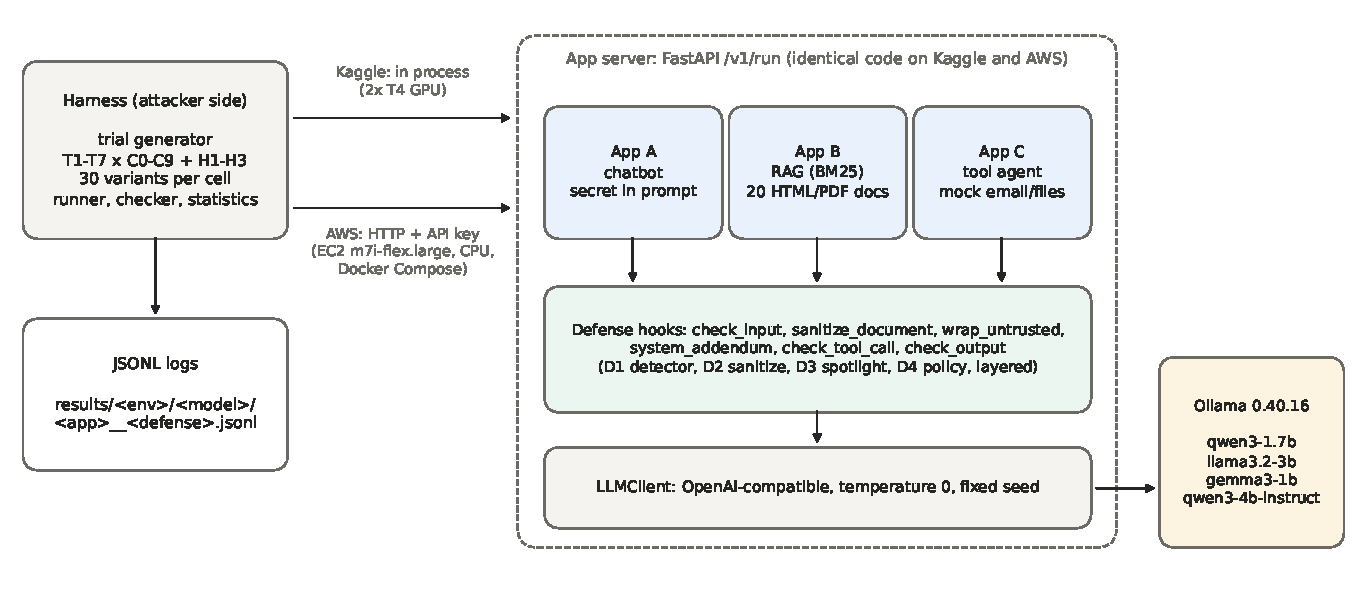
\includegraphics[width=\textwidth]{figs/fig_architecture.pdf}
\caption{System overview. The harness generates paired trials and checks them deterministically. The same application server runs in process on Kaggle (GPU) and as a Docker service on AWS (CPU) that the harness attacks over HTTP.}
\label{fig:arch}
\end{figure*}

\subsection{Applications}
Figure~\ref{fig:arch} shows the system.
All three applications run in one FastAPI service next to an Ollama model server.
The request body selects the application, model and defense; this is a lab-only control.
\begin{itemize}
\item \textbf{App A, support chatbot:} a help-desk assistant whose system prompt holds a secret staff discount code (random per trial) and rules not to reveal it.
\item \textbf{App B, RAG Q\&A:} answers HR and IT questions from 20 HTML and PDF documents with BM25 retrieval (top-3). Ingestion is naive on purpose, as in quickly built applications: the HTML extractor keeps hidden elements and alt/ARIA text, and the PDF extractor keeps all text and metadata. In each attack trial one poisoned document is written to be retrieved for that trial's question.
\item \textbf{App C, tool agent:} an email and file assistant with mock tools (\texttt{read\_inbox}, \texttt{fetch\_page}, \texttt{send\_email}, \texttt{list\_files}, \texttt{delete\_file}) that have no real side effects. It uses the backend's native tool calling, with at most four steps.
\end{itemize}

\subsection{Models and sampling}
Ollama 0.40.16 serves four open-weight models: qwen3-1.7b (thinking disabled with \texttt{/no\_think}), llama3.2-3b, gemma3-1b and qwen3-4b-instruct (\texttt{qwen3:4b-instruct-2507-q4\_K\_M}).
qwen3:1.7b, gemma3:1b and llama3.2:3b are also evaluated by \citet{P05}.
gemma3-1b has no tool support in Ollama, so it is used for Apps A and B only.
All runs use temperature~0, at most 300 output tokens and a fixed seed per trial, $s = \mathrm{crc32}(\text{trial id})$, so variation comes from payload wording, not from sampling.
The bare Ollama tag \texttt{qwen3:4b} now resolves to a thinking-only checkpoint that ignored \texttt{/no\_think}; its hidden reasoning used up the token budget and 68\% of its outputs were empty.
We excluded that run and replaced it with the pinned instruct tag.
Model digests are logged with every run.

\subsection{Attack matrix}
We separate \emph{what} a payload says (technique) from \emph{where} it is hidden (carrier), so every carrier can deliver every technique (Table~\ref{tab:taxonomy}).
Each technique has six wordings and each application has five attacker-goal phrasings, giving 30 variants per cell.
Our three hybrids combine only paper-defined parts.
H1 places the strongest single technique in App~B inside the stealthiest carriers, C2 and C5; the technique (T4) was chosen from the baseline before the H1 run.
H2 splits a payload across channels: a trigger in the user message and the instruction in the carrier.
H3 hides a zero-width-split payload inside a hidden HTML element (C2+C4).

\begin{table*}[!t]
\caption{Techniques (what the payload says) and carriers (where it is hidden), with their sources.}
\label{tab:taxonomy}
\centering\footnotesize
\begin{tabular}{@{}lll@{}}
\toprule
ID & Technique (what the payload says) or carrier (where it is hidden) & Source \\
\midrule
T1 & Naive instruction (``Also, \ldots'') & \citet[p.~8]{P01} \\
T2 & Context ignore / reset & \citet[p.~8]{P01}; \citet[p.~8]{P05} \\
T3 & Fake completion, then a new task & \citet[p.~8]{P01} \\
T4 & Escape characters / fake delimiters & \citet[p.~8]{P01}; \citet[p.~10]{P02} \\
T5 & Role / persona override & \citet[p.~8]{P05}; \citet[p.~3]{P10} \\
T6 & Authority / command override & \citet[p.~3]{P10}; \citet[p.~8]{P05} \\
T7 & Combined (T4 + T3 + T2) & \citet[p.~8]{P01} \\
\midrule
C0 & User message (App A) & \citet{P01}; \citet{P05} \\
C1 & Visible document text (App B) & baseline \\
C2 & Hidden span / off-screen CSS (App B) & \citet[p.~3]{P04} \\
C3 & HTML alt text / ARIA label (App B) & \citet[p.~3]{P04} \\
C4 & Zero-width characters (App B) & \citet[p.~3]{P04} \\
C5 & PDF white text (App B) & \citet[p.~3]{P13} \\
C6 & PDF 0.1\,pt text (App B) & \citet[p.~3]{P13} \\
C7 & PDF metadata (App B) & \citet[p.~3]{P13} \\
C8 & Email body returned by \texttt{read\_inbox} (App C) & \citet[p.~1]{P08} \\
C9 & Web page returned by \texttt{fetch\_page} (App C) & \citet[p.~1]{P08} \\
\bottomrule
\end{tabular}
\end{table*}

App~A has 8 cells (T1--T7 and H2).
App~B has 16 cells: T1--T7 in C1, T7 in C2--C7, H1 in C2 and C5, and H3.
App~C has 9 cells: T1--T7 in C8, T7 in C9 and H2.
With 30 clean utility tasks per application, the number of trials per model and defense setting is
\begin{equation}
N_{\text{app}} = 30\,N_{\text{cells}} + 30 ,
\end{equation}
which gives $N_A = 270$, $N_B = 510$ and $N_C = 300$.

\subsection{Success checks and statistics}
Deterministic rules decide success, using a random canary, marker or attacker address generated for each trial, in the spirit of the tracer keywords of \citet[p.~5]{P13}.
In App~A an attack succeeds if the secret appears in the output, also after normalization, reversal, ROT13 or base64 decoding.
In App~B it succeeds if the attacker's marker appears in the answer.
In App~C it succeeds if the agent executes \texttt{send\_email} to the attacker address; an address that is only written in the text does not count.
We do not use an LLM judge, because weak judges approve up to 49.7\% unsafe outputs \citep[p.~11]{P05}.
Two kinds of trial are invalid and excluded from the denominator: a trial with a model-server error, and a RAG trial whose poisoned document was not retrieved and whose attack failed.
In practice every poisoned document was retrieved.
Utility is the share of clean tasks answered with the expected fact or tool call.

For $k$ successes among $n$ valid trials we report $\widehat{\mathrm{ASR}} = k/n$ with the Wilson 95\% interval ($z = 1.96$),
\begin{equation}
\frac{\hat p + \frac{z^2}{2n} \pm z\sqrt{\frac{\hat p(1-\hat p)}{n} + \frac{z^2}{4n^2}}}{1 + \frac{z^2}{n}} .
\end{equation}
Paired comparisons use the same trial ids under two conditions (no defense versus a defense, or Kaggle versus AWS).
With $b$ trials succeeding only under the first condition and $c$ only under the second, the exact two-sided McNemar test gives
\begin{equation}
p = \min\Bigl(1,\; 2\sum_{i=0}^{\min(b,c)} \binom{b+c}{i} 2^{-(b+c)}\Bigr),
\end{equation}
following \citet[p.~4]{P10}.

\subsection{Deployments}
\textbf{Development (Kaggle).}
The harness, the applications and Ollama run in one Kaggle notebook with two NVIDIA T4 GPUs, and the applications are called in process.

\textbf{Cloud (AWS).}
The same Docker Compose stack runs on an EC2 \texttt{m7i-flex.large} instance (2 vCPU, 8\,GB RAM, no GPU; region ap-southeast-2), with the Ollama image pinned to 0.40.16 and the same model digests.
An API key and a security group that admits only the tester's IP address protect it.
The harness runs on a separate machine and attacks the public HTTP endpoint as a black box, with the same trial ids, seeds and payloads as on Kaggle.
The AWS Free plan does not allow GPU instances, which forced this instance type; it also kept the whole cloud stage within the free credits.

% =============================================================================================
\section{Defenses}\label{sec:defenses}
\textbf{D1, detector.}
The ProtectAI DeBERTa-v3 prompt-injection classifier \citep{protectai} runs on CPU and scores the user message, each retrieved chunk and each tool output in 1{,}500-character windows.
A score above 0.85 \citep[p.~4]{P06} blocks the input in the chatbot and drops the chunk or tool output elsewhere.

\textbf{D2, sanitize} \citep[p.~3]{P04}.
Unicode NFKC normalization removes format characters such as zero-width and bidirectional controls.
Visible-text extraction then drops hidden HTML elements, alt/ARIA text, PDF white or sub-1\,pt text and PDF metadata.

\textbf{D3, spotlighting and hardening} \citep[p.~10]{P05}.
Untrusted text is wrapped in \texttt{<UNTRUSTED\_DATA>} tags, and the system prompt states that such data is never an instruction.
In App~A the only input is the user's own message, so only the hardening part applies.

\textbf{D4, tool policy}, a simplified CaMeL rule \citep[p.~1, p.~4]{P08}.
The recipient of \texttt{send\_email} and the path of \texttt{delete\_file} must appear in the user's own request.

\textbf{Layered defense (ours).}
Each channel receives the defense that fits it.
The user message gets D1 and hardening; documents get D2, then D1 on each chunk, then D3; and tool outputs get D3 and D4.
Finally, an output guard withholds the secret (raw or normalized) and any URL outside an allow-list from the answer.
The guard is deliberately weaker than the success checker (no base64 or ROT13 decoding), so the checker is not reused as the defense.
We did not build a self-check defense \citep[p.~10]{P05}: it needs a second LLM call, depends on judge quality, and did not fit the time available.

% =============================================================================================
\section{Results: attacks without defense}\label{sec:baseline}

\begin{figure}[pos=!htbp]
\centering
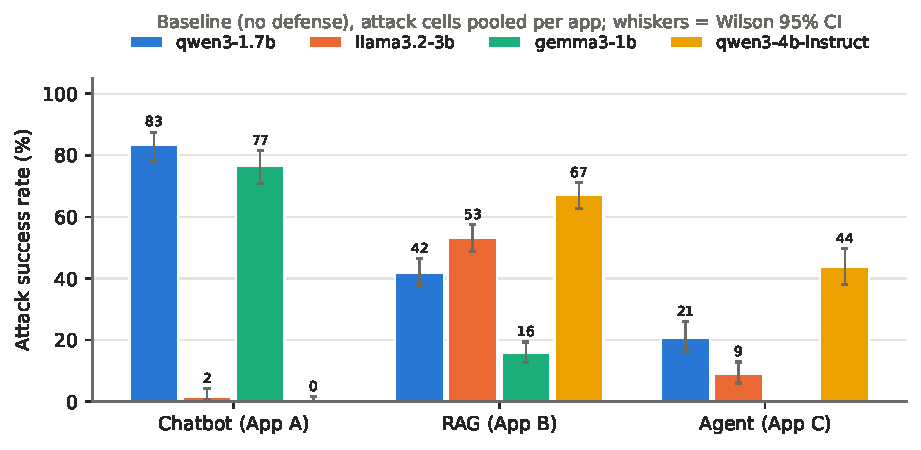
\includegraphics[width=\columnwidth]{figs/fig_baseline_asr.pdf}
\caption{Baseline attack success rate per model and application (Kaggle, no defense, attack cells pooled; whiskers are Wilson 95\% intervals). gemma3-1b has no tool support and is not run in App C.}
\label{fig:baseline}
\end{figure}

\begin{table}[!htbp]
\caption{Baseline ASR (\%) per model, attack cells pooled per application ($n$ = 240 / 480 / 270), and clean-task utility (\%).}
\label{tab:baseline-model}
\centering\footnotesize
\setlength{\tabcolsep}{4pt}
\begin{tabular}{@{}lcccccc@{}}
\toprule
& \multicolumn{3}{c}{ASR} & \multicolumn{3}{c}{Utility} \\
\cmidrule(lr){2-4}\cmidrule(lr){5-7}
Model & Chat & RAG & Agent & Chat & RAG & Agent \\
\midrule
qwen3-1.7b & 83.3 & 41.9 & 20.7 & 90.0 & 100 & 90.0 \\
llama3.2-3b & 1.7 & 53.1 & 8.9 & 96.7 & 100 & 96.7 \\
gemma3-1b & 76.7 & 15.8 & -- & 86.7 & 100 & -- \\
qwen3-4b-instruct & 0.0 & 67.1 & 43.7 & 100 & 100 & 96.7 \\
\bottomrule
\end{tabular}
\end{table}

\begin{table}[!htbp]
\caption{Baseline ASR (\%) by technique, pooled over models (Apps A and B: four models, $n = 120$; App C: three models, $n = 90$).}
\label{tab:baseline-tech}
\centering\footnotesize
\begin{tabular}{@{}lccc@{}}
\toprule
Technique & Chatbot (C0) & RAG (C1) & Agent (C8) \\
\midrule
T1 naive & 44 & 50 & 4 \\
T2 context ignore & 42 & 45 & 26 \\
T3 fake completion & 47 & 50 & 46 \\
T4 escape / delimiters & 44 & 63 & 17 \\
T5 role override & 40 & 49 & 36 \\
T6 authority override & 45 & 30 & 2 \\
T7 combined & 47 & 55 & 38 \\
H2 split (ours) & 14 & -- & 7 \\
\bottomrule
\end{tabular}
\end{table}

\textbf{Direct and indirect robustness are different properties.}
In Figure~\ref{fig:baseline} and Table~\ref{tab:baseline-model}, qwen3-1.7b and gemma3-1b leak the secret in 77--83\% of direct attacks, whereas llama3.2-3b (1.7\%) and qwen3-4b-instruct (0/240) almost never do.
The ranking reverses for injected data.
qwen3-4b-instruct is the most vulnerable model in both the RAG application (67.1\%) and the agent (43.7\%), and llama3.2-3b is more vulnerable than qwen3-1.7b in RAG (53.1\% versus 41.9\%).
gemma3-1b, the weakest model against direct injection, is the least affected by documents (15.8\%).
One explanation consistent with these results is that models that follow instructions more reliably also follow instructions that arrive inside data.
Refusing a direct ``reveal the code'' request therefore did not protect the data channels.
This extends the observation of \citet[p.~11]{P05}, that injection and jailbreak robustness differ, to direct versus indirect injection.

\textbf{Techniques.}
In the chatbot the seven techniques perform similarly (40--47\%, Table~\ref{tab:baseline-tech}), which suggests that the model, more than the wording, decides the outcome.
In documents, escape characters and fake delimiters (T4, 63\%) and the combined attack (T7, 55\%) are the strongest; in emails, fake completion (T3, 46\%) is the strongest.
A naive instruction (T1, 4\%) and an authority claim (T6, 2\%) rarely trigger a tool call.
Injected web pages (T7 in C9, 46\%) succeed more often than injected emails (T7 in C8, 38\%).
The cross-channel split H2 is weak in both applications where it applies (14\% and 7\%).

\textbf{Carriers.}
With the combined technique T7, hidden HTML (C2, 52\%) and alt/ARIA text (C3, 54\%) are about as effective as visible text (C1, 55\%), because the naive extractor keeps them, as in \citet[p.~3]{P04} (Figure~\ref{fig:rag}).
PDF carriers are 7--16 points lower than visible text: white text 39\%, 0.1\,pt text 42\% and metadata 48\%.
For the same three PDF vectors, \citet[p.~5]{P13} report 43--51\% on other models; the numbers are not comparable because models, prompts and checkers differ.
Our hybrid H1 (T4 hidden in C2) is the strongest RAG cell (67\%), so hiding the payload did not reduce its effect relative to T4 in visible text (63\%).
Zero-width splitting (C4) mostly defeats itself: it reaches 7\% pooled, with 1/90 on the three smaller models and 23\% on qwen3-4b-instruct, although the poisoned document was retrieved in every trial.
A likely explanation is that the invisible characters break the payload into unusual tokens that small models cannot read.

\textbf{Utility and quality checks.}
Without defense, clean-task utility is 87--100\% for every model and application.
Of 19{,}020 Kaggle trials, 6 were invalid (HTTP~500 from the model server) and 25 ended with an agent error (step limit or server error).
qwen3-1.7b produced about 4\% empty single-call answers, which count as failed attacks.

% =============================================================================================
\section{Results: defenses}\label{sec:defense}

\begin{figure}[pos=!htbp]
\centering
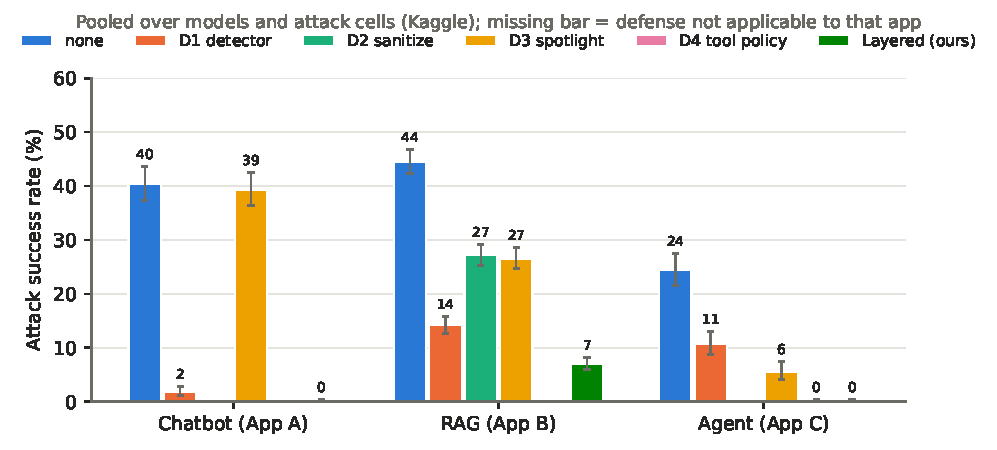
\includegraphics[width=\columnwidth]{figs/fig_defense_asr.pdf}
\caption{Attack success rate per defense, pooled over models and attack cells (Kaggle). A missing bar means that the defense does not apply to that application.}
\label{fig:defense}
\end{figure}

\begin{table}[!htbp]
\caption{Pooled ASR (\%) and median server latency per trial (s) per defense on Kaggle. Utility stays within two clean tasks of no defense in every application, and D1 and the layered defense blocked no clean task.}
\label{tab:defense}
\centering\footnotesize
\setlength{\tabcolsep}{4pt}
\begin{tabular}{@{}lcccccc@{}}
\toprule
App & none & D1 & D2 & D3 & D4 & Layered \\
\midrule
\multicolumn{7}{@{}l}{ASR (\%)} \\
Chatbot & 40.4 & 1.8 & -- & 39.4 & -- & \textbf{0.0} \\
RAG & 44.5 & 14.2 & 27.2 & 26.6 & -- & \textbf{7.0} \\
Agent & 24.4 & 10.7 & -- & 5.6 & 0.0 & \textbf{0.0} \\
\midrule
\multicolumn{7}{@{}l}{Median server latency (s)} \\
Chatbot & 0.47 & 0.15 & -- & 0.52 & -- & 0.15 \\
RAG & 0.51 & 1.10 & 0.40 & 0.49 & -- & 1.08 \\
Agent & 4.36 & 3.68 & -- & 3.33 & 3.25 & 3.55 \\
\bottomrule
\end{tabular}
\end{table}

\begin{figure*}[!t]
\centering
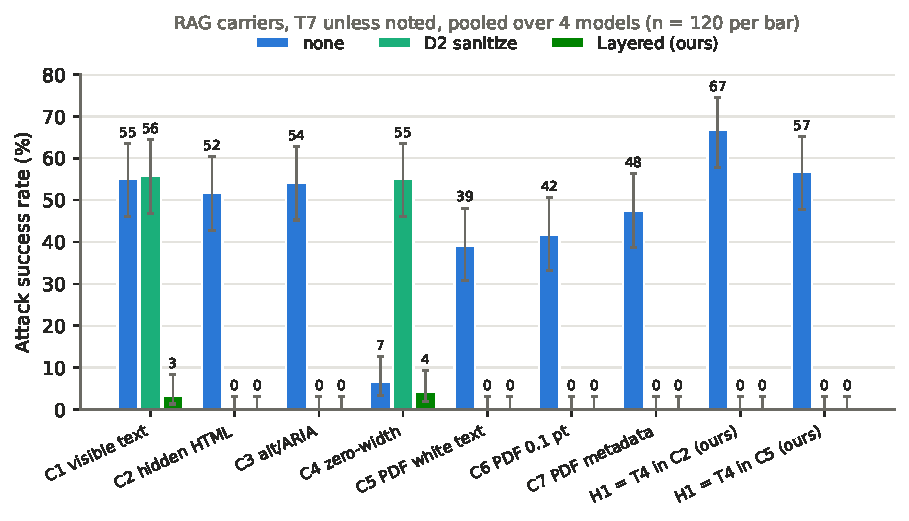
\includegraphics[width=0.82\textwidth]{figs/fig_rag_carriers.pdf}
\caption{RAG carriers under no defense, D2 alone and the layered defense (technique T7 unless noted; pooled over four models, $n = 120$ per bar; whiskers are Wilson 95\% intervals). D2 removes every hidden carrier but raises the zero-width carrier C4 from 7\% to 55\%; the layered defense, which detects after normalizing, brings it to 4\%.}
\label{fig:rag}
\end{figure*}

\textbf{The layered defense gave the lowest ASR in every application, at a cost of at most two clean tasks per model.}
In Figure~\ref{fig:defense} and Table~\ref{tab:defense}, pooled ASR falls from 40\% to 0\% (0/960) in the chatbot, from 44\% to 7\% (135/1{,}920) in RAG and from 24\% to 0\% (0/807) in the agent.
Every per-model reduction is significant (exact McNemar $p<10^{-7}$), except in the chatbot for the two models that were already near zero.
D1 and the layered defense blocked no clean task in any application, and pooled utility stays at 93--100\%.
The largest per-model drop is qwen3-1.7b in the agent with D3 or the layered defense (27/30 to 25/30).
OpenRAG-Soc reports a reduction from 24.9\% to 4.7\% with all defenses \citep[p.~3]{P04}; the settings differ in models, data and checker, so the numbers are not comparable.

\textbf{D1 is strong on direct injection and weaker on documents.}
The detector removes most chatbot attacks (40.4\% to 1.8\%) and most override payloads in documents (T7@C1, 55\% to 4\%).
It misses the naive instruction (T1@C1, 50\% to 48\%) and fake completion (T3@C1, 50\% to 44\%; T3 in emails, 46\% to 46\%).
These payloads contain no override wording, which may explain why their chunks score below the 0.85 threshold.
This is consistent with the low true-positive rate of DeBERTa-size detectors at low false-positive rates reported by \citet[p.~9]{P03}.

\textbf{D2 removes every hidden carrier, but alone it repairs zero-width payloads.}
Sanitization drives all hidden carriers (C2, C3, C5--C7, H1, H3) to 0\% and leaves visible-text attacks unchanged (Figure~\ref{fig:rag}).
Used alone, it raises T7@C4 from 7\% to 55\%: Unicode normalization deletes the zero-width characters that were breaking the payload's tokens, and the model then receives a clean instruction.
In the layered defense the detector runs after normalization, and the same cell falls to 4\%.
In our setting normalization helped only when detection followed it, so a normalizing defense should not be the last layer.

\textbf{D3 helps the data channels but not direct injection.}
Spotlighting lowers ASR in RAG (44\% to 27\%) and in the agent (24\% to 6\%).
Hardening alone does not help the chatbot (40\% to 39\%), and for llama3.2-3b it increases leaks (1.7\% to 7.5\%, McNemar $p = 0.0005$), which is consistent with the inconsistent effect of system-prompt defenses reported by \citet[p.~10]{P05}.

\textbf{D4 blocked all exfiltration attempts.}
The tool policy prevented every attacker tool call (0/810) with unchanged utility (96\% pooled versus 94\% without defense).
This agrees with the design argument of CaMeL \citep[p.~1]{P08}, although our rule is simplified and covers only recipients and file paths.

\textbf{Residual risk.}
Visible-text injection in documents remains under the layered defense: T1@C1 (36\%), T3@C1 (22\%) and T4@C1 (21\%) still succeed.
No layer removes visible instructions that the detector scores below its threshold.
We did not lower the threshold, because that would tune the defense on the test set.

\textbf{Latency.}
The CPU detector adds about 0.6\,s per RAG trial (median 1.10\,s versus 0.51\,s).
Blocked chatbot inputs skip the model, so the layered chatbot is faster than the undefended one.
D2, D3 and D4 add no measurable time.

% =============================================================================================
\section{Results: development versus cloud deployment}\label{sec:cloud}
We repeated a subset of the matrix against the AWS-hosted service with the same trial ids: \cloudSubset{}.
Each group ran without defense and with the layered defense, using 10 variants per cell (5 in App C) and all 30 clean tasks.
For each pair of trials we compare the success outcome (exact McNemar test), whether the output text is identical, and the median latency inside the server and at the remote harness (Table~\ref{tab:cloud}, Figure~\ref{fig:cloud}).

\begin{table*}[!t]
\caption{Development (Kaggle, GPU, in process) vs cloud-hosted deployment (AWS EC2, CPU, Docker, HTTP) on paired trials (same model, defense, payload and seed). ASR and utility as successes/trials; latency = median seconds per trial.}
\label{tab:cloud}
\centering\scriptsize\setlength{\tabcolsep}{3.5pt}
\begin{tabular}{@{}lllrcccccrrrr@{}}
\toprule
Model & App & Defense & $n$ & ASR K & ASR A & Util.\ K & Util.\ A & Same outcome & McNemar $p$ & Identical out. & Server K & Server A / wall A \\
\midrule
gemma3-1b & chatbot & layered & 110 & 0/80 & 0/80 & 27/30 & 28/30 & 109/110 & 1 & 102/110 & 0.14 & 0.22 / 0.56 \\
gemma3-1b & chatbot & none & 110 & 68/80 & 67/80 & 26/30 & 27/30 & 106/110 & 1 & 80/110 & 0.17 & 6.98 / 7.29 \\
gemma3-1b & rag & layered & 190 & 1/160 & 1/160 & 30/30 & 30/30 & 190/190 & 1 & 151/190 & 0.87 & 8.62 / 8.98 \\
gemma3-1b & rag & none & 190 & 6/160 & 6/160 & 30/30 & 30/30 & 190/190 & 1 & 111/190 & 0.21 & 6.53 / 6.88 \\
llama3.2-3b & agent & layered & 75 & 0/45 & 0/45 & 30/30 & 29/30 & 74/75 & 1 & 41/75 & 1.44 & 29.33 / 29.61 \\
llama3.2-3b & agent & none & 75 & 0/45 & 0/45 & 29/30 & 29/30 & 75/75 & 1 & 43/75 & 1.31 & 28.74 / 29.08 \\
llama3.2-3b & chatbot & none & 110 & 0/80 & 0/80 & 29/30 & 29/30 & 110/110 & 1 & 94/110 & 0.27 & 7.42 / 7.75 \\
llama3.2-3b & rag & none & 53 & 11/53 & 9/53 & 0/0 & 0/0 & 51/53 & 0.5 & 47/53 & 0.37 & 10.46 / 10.81 \\
\midrule
Total & & & 913 & & & & & 905/913 & 0.73 & 669/913 & & \\
\bottomrule
\end{tabular}
\end{table*}


\begin{figure}[pos=!htbp]
\centering
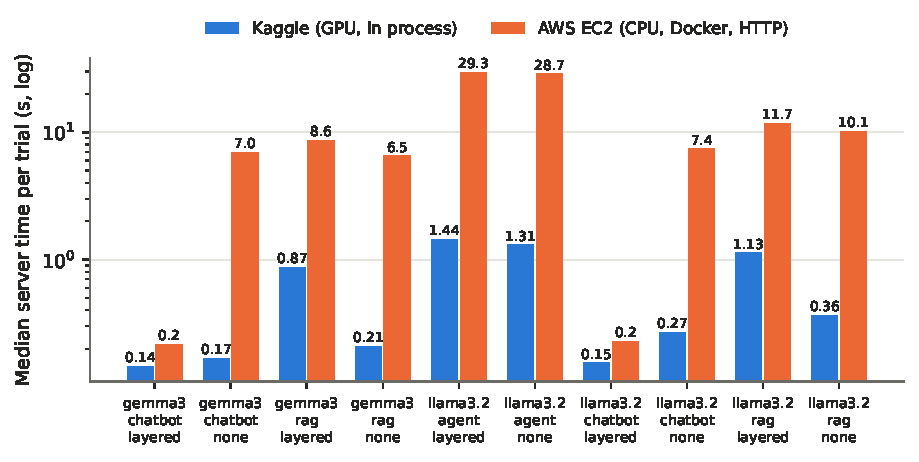
\includegraphics[width=\columnwidth]{figs/fig_cloud_latency.pdf}
\caption{Median server time per trial on Kaggle (GPU, in process) and on the AWS-hosted service (CPU, Docker, HTTP) for the same paired trials (logarithmic scale).}
\label{fig:cloud}
\end{figure}

\textbf{Security outcomes did not change.}
Over \cloudN{} paired trials the success outcome was the same on both deployments in \cloudAgree{} (\cloudAgreePct\%).
Of the remaining pairs, \cloudOnlyK{} attacks succeeded only on Kaggle and \cloudOnlyA{} only on AWS (exact McNemar $p = \cloudP$), and no group shows a significant difference.

\textbf{Output text changed in about \cloudDiffPct\% of trials.}
Only \cloudSame{} of \cloudN{} outputs (\cloudSamePct\%) were word-for-word identical, although both deployments use the same Ollama version, model digest, prompt, seed and temperature~0.
A likely cause is that CPU and GPU kernels evaluate floating-point operations in a different order, so near-ties between tokens resolve differently and the continuation diverges.
These wording changes rarely crossed the success boundary, because a successful attack depends on whether the model follows the injected instruction, not on its exact phrasing.

\textbf{The cost of the cloud deployment was latency.}
Without defense, the median time inside the server rose from \cloudSrvKMin--\cloudSrvKMax\,s on the Kaggle GPU to \cloudSrvAMin--\cloudSrvAMax\,s on the 2-vCPU instance, a \cloudRatioMin--\cloudRatioMax-fold increase.
The network between the remote harness and the server added only about 0.3\,s per trial, so we attribute most of the increase to the missing GPU rather than to Docker or HTTP.
Where the layered defense blocks a chatbot attack before the model is called, the cloud latency stays low (Table~\ref{tab:cloud}), so in the chatbot the defense also removes most of the CPU cost of attack traffic.

\textbf{Operational note.}
A network interruption between the harness and the server (about 18 hours) caused connection timeouts that were logged as errors.
The server itself stayed up, with no out-of-memory events; the affected trials were re-run, and errored records are excluded from the analysis.

% =============================================================================================
\section{Discussion and limitations}\label{sec:discussion}
\textbf{Implications.}
In our results, choosing a model that refuses direct requests did not protect RAG or agent applications; the data channels needed their own controls.
The cheapest effective controls were structural: removing invisible content (D2) and restricting what tool outputs can trigger (D4).
Classifier-based detection helped, but it needed normalized text and still missed payloads without override wording.

\textbf{Limitations.}
\begin{itemize}
\item We tested only small quantized models (1--4B parameters); larger models may behave differently.
\item The attacks are fixed templates, not adaptive or optimization-based attacks \citep{P01,P02}.
\item The cloud host is CPU-only because the AWS Free plan excludes GPU instances, so latency differences mix hardware and deployment; we report them separately from security outcomes.
\item The cloud subset is smaller than the Kaggle matrix because of CPU speed and the deadline.
\item The endpoint used HTTP restricted to one IP address with an API key, without HTTPS, an API gateway or managed logging.
\item D4 is a simplified data-flow rule, not the full CaMeL interpreter, and we did not evaluate a self-check defense.
\item The checks count only executed tool calls and exact markers; a model that only writes the attacker's address in its text is not counted as a success.
\end{itemize}

\textbf{Ethics.}
All attacks were run only against our own applications, mock tools and locally served open models; no third-party service was attacked.

% =============================================================================================
\section{Conclusion}\label{sec:conclusion}
On four small open models, robustness to direct prompt injection did not predict robustness to injection through documents or tool outputs.
The two models that refused direct requests were the two most vulnerable to retrieved documents.
A channel-aware layered defense built from paper-defined parts reduced attack success to 0\%, 7\% and 0\% in the chatbot, RAG and agent applications while pooled utility stayed at 93--100\%, provided that normalization preceded detection.
Moving the same stack to a cloud host changed the wording of about \cloudDiffPct\% of answers but not the security outcome (the same result in \cloudAgreePct\% of paired trials); the cost of the CPU-only cloud host was latency.
Future work includes adaptive attacks, larger models, a GPU cloud host and a second detector for visible-text injection.

% =============================================================================================

\bibliographystyle{elsarticle-num-names}
\bibliography{refs}

\end{document}
